\documentclass{beamer}
\usetheme{ConnectivityLab}
\usepackage{times}
\usepackage{graphicx}
\usepackage{verbatim}
\usepackage{outlines}
\usepackage{fancyhdr}
\usepackage{subfigure}
\usepackage{cancel}
\usepackage{bibentry}
\usepackage{varwidth}
\usepackage{etoolbox}
\usepackage{epstopdf}

%%%%%%%%%%%%%%%%%%%%%%%%%%%%%%%%%%%%%%%%%%%%%%%%%%%%%%
%%%%%%%%%%%%%%%%%%%%%%%%%%%%%%%%%%%%%%%%%%%%%%%%%%%%%%

\title {
    Progress report
}
\author {
    Speaker: Hsu, Yin-Hong
}
\date {
    12 22, 2016 %\today
}

%%%%%%%%%%%%%%%%%%%%%%%%%%%%%%%%%%%%%%%%%%%%%%%%%%%%%%
%%%%%%%%%%%%%%%%%%%%%%%%%%%%%%%%%%%%%%%%%%%%%%%%%%%%%%

\begin{document}
\begin{frame}
    \titlepage
\end{frame}

%%%%%%%%%%%%%%%%%%%%%%%%%%%%%%%%%%%%%%%%%%%%%%%%%%%%%%
%%%%%%%%%%%%%%%%%%%%%%%%%%%%%%%%%%%%%%%%%%%%%%%%%%%%%%

\begin{frame}{Outline}
    \tableofcontentsgather
    \tableofcontents
\end{frame}

%%%%%%%%%%%%%%%%%%%%%%%%%%%%%%%%%%%%%%%%%%%%%%%%%%%%%%
%%%%%%%%%%%%%%%%%%%%%%%%%%%%%%%%%%%%%%%%%%%%%%%%%%%%%%
\section{My Work}

%%%%%%%%%%%%%%%%%%%%%%%%%%%%%%%%%%%%%%%%%%%%%%%%%%%%%%
%%%%%%%%%%%%%%%%%%%%%%%%%%%%%%%%%%%%%%%%%%%%%%%%%%%%%%
\begin{frame}{Simulation structure}
    \begin{figure}[t]
        \centering
        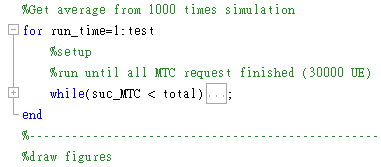
\includegraphics[width=0.9\textwidth]{figures/intro.png}
        \setbeamerfont{caption}{size=\tiny}
        \caption{structure}
    \end{figure}
\end{frame}

%%%%%%%%%%%%%%%%%%%%%%%%%%%%%%%%%%%%%%%%%%%%%%%%%%%%%%
%%%%%%%%%%%%%%%%%%%%%%%%%%%%%%%%%%%%%%%%%%%%%%%%%%%%%%
\begin{frame}{Performance Optimization}
    \begin{itemize}
        \item {for loop $\rightarrow$ Vectorized}
        \item {unique function $\rightarrow$ find/sort/diff}
        \item {remove redundant code}
        \item {predefine variables}
        \item {parallel/gpu but failed}
    \end{itemize}
\end{frame}

%%%%%%%%%%%%%%%%%%%%%%%%%%%%%%%%%%%%%%%%%%%%%%%%%%%%%%
%%%%%%%%%%%%%%%%%%%%%%%%%%%%%%%%%%%%%%%%%%%%%%%%%%%%%%
\section{Result}

%%%%%%%%%%%%%%%%%%%%%%%%%%%%%%%%%%%%%%%%%%%%%%%%%%%%%%
%%%%%%%%%%%%%%%%%%%%%%%%%%%%%%%%%%%%%%%%%%%%%%%%%%%%%%
\begin{frame}{Compare - time cost with some minor fix}
    \begin{center}
        \begin{tabular}{|c|c|c|}
        \hline
        \textbf{}          & \textbf{before (1 run)} & \textbf{after (1 run)} \\ \hline
        \textbf{time}      & \textbf{563s}   & \textbf{362s}  \\ \hline
        \textbf{propotion} & \textbf{100\%}  & \textbf{64\%}  \\ \hline
        \end{tabular}
    \end{center}
\end{frame}

\begin{frame}{Compare - time cost with spmd}
    \begin{center}
        \begin{tabular}{|c|c|c|}
        \hline
        \textbf{}          & \textbf{before (1 run)} & \textbf{after (4 run)} \\ \hline
        \textbf{time}      & \textbf{563s}   & \textbf{447s}  \\ \hline
        \textbf{propotion} & \textbf{100\%}  & \textbf{20\%}  \\ \hline
        \end{tabular}
    \end{center}
\end{frame}
%%%%%%%%%%%%%%%%%%%%%%%%%%%%%%%%%%%%%%%%%%%%%%%%%%%%%%
%%%%%%%%%%%%%%%%%%%%%%%%%%%%%%%%%%%%%%%%%%%%%%%%%%%%%%
\begin{frame}{Simulation result - past}
    \begin{figure}[t]
        \centering
        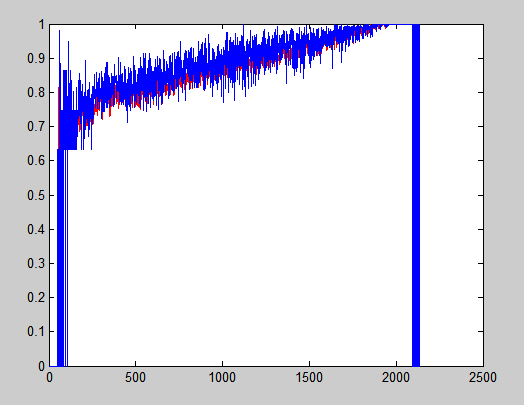
\includegraphics[width=0.7\textwidth]{figures/past.png}
        \setbeamerfont{caption}{size=\tiny}
        \caption{structure}
    \end{figure}
\end{frame}

\begin{frame}{Simulation result - new}
    \begin{figure}[t]
        \centering
        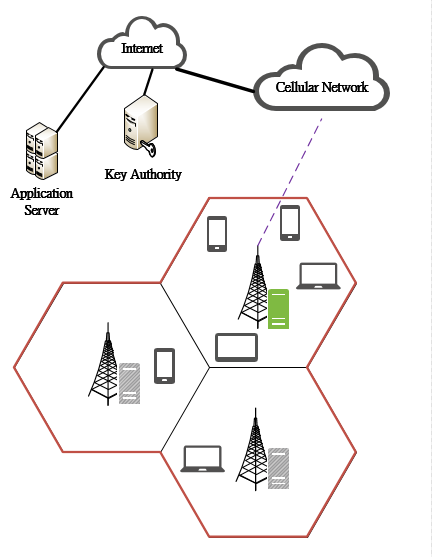
\includegraphics[width=0.7\textwidth]{figures/new.png}
        \setbeamerfont{caption}{size=\tiny}
        \caption{structure}
    \end{figure}
\end{frame}

\begin{frame}{Future work and problems}
    \begin{itemize}
        \item {fix some bug}
        \item {Adjust the simulation variable to compare with other paper}
        \item {no script to draw the figure in Simulation result section}
    \end{itemize}
\end{frame}

%%%%%%%%%%%%%%%%%%%%%%%%%%%%%%%%%%%%%%%%%%%%%%%%%%%%%%
%%%%%%%%%%%%%%%%%%%%%%%%%%%%%%%%%%%%%%%%%%%%%%%%%%%%%%

\section{}

\begin{frame}
    \centering
    \Large{Thanks for Your Attentions}
\end{frame}

\end{document}
